\documentclass[11pt]{article}

% some definitions for the title page
\newcommand{\reporttitle}{example}
\newcommand{\reportdescription}{example description}

% load some definitions and default packages
%---------------------------------------------------------------------------
%	PACKAGES AND OTHER DOCUMENT CONFIGURATIONS
%---------------------------------------------------------------------------

\usepackage[twoside]{fancyhdr}
\usepackage{csquotes}

\usepackage[a4paper,hmargin=2.0cm,vmargin=1.0cm,includeheadfoot]{geometry}
% \usepackage{natbib} % for bibliography
\usepackage{biblatex}
\usepackage{tabularx,longtable,multirow,subfigure,caption}%hangcaption
\usepackage{fancyhdr} % page layout
\usepackage{url} % URLs
\usepackage[english]{babel}
\usepackage{graphicx}
\usepackage{rotating}
\usepackage{dsfont}
\usepackage{epstopdf} % automatically replace .eps with .pdf in graphics
% \usepackage{backref} % needed for citations
\usepackage{array}
\usepackage{latexsym}
\usepackage[pdftex,hypertexnames=false,colorlinks]{hyperref} % provide links in pdf (had pagebackref)
\usepackage{booktabs}
\usepackage{wrapfig}
\usepackage{caption}  % Required for \captionof
\usepackage{float} % for H option in figures
\usepackage{amssymb}
\usepackage{amsmath}
\usepackage{amsthm}
\usepackage{mathtools} % for 'dcases*' env.
\usepackage[nottoc]{tocbibind}

%%% Default fonts
\renewcommand*{\rmdefault}{bch}
\renewcommand*{\ttdefault}{cmtt}

%%% Default settings (page layout)
\setlength{\parindent}{0em}  % indentation of paragraph
\setlength{\parskip}{.3em}
\setlength{\itemsep}{0.mm}

\setlength{\headheight}{14.5pt}
\pagestyle{fancy}

\fancyfoot[ER,OL]{\thepage}%Page no. in the left on odd pages and on right on even pages

\fancyfoot[OC,EC]{\sffamily }
\renewcommand{\headrulewidth}{0.1pt}
\renewcommand{\footrulewidth}{0.1pt}
\captionsetup{margin=10pt,font=small,labelfont=bf}

% LISTINGS ammendments
\usepackage{listings}
\usepackage{color}

\definecolor{mygreen}{rgb}{0,0.6,0}
\definecolor{mygray}{rgb}{0.5,0.5,0.5}
\definecolor{mymauve}{rgb}{0.58,0,0.82}

\lstset{ 
  postbreak=\mbox{\textcolor{red}{$\hookrightarrow$}\space},
  backgroundcolor=\color{white},   % choose the background color; you must add \usepackage{color} or \usepackage{xcolor}; should come as last argument
  basicstyle=\footnotesize,        % the size of the fonts that are used for the code
  breakatwhitespace=false,         % sets if automatic breaks should only happen at whitespace
  breaklines=true,                 % sets automatic line breaking
  captionpos=b,                    % sets the caption-position to bottom
  commentstyle=\color{mygreen},    % comment style
%   deletekeywords={...},            % if you want to delete keywords from the given language
%   escapeinside={\%*}{*)},          % if you want to add LaTeX within your code
  extendedchars=true,              % lets you use non-ASCII characters; for 8-bits encodings only, does not work with UTF-8
  firstnumber=1,                % start line enumeration with line 1000
  frame=single,	                   % adds a frame around the code
  keepspaces=true,                 % keeps spaces in text, useful for keeping indentation of code (possibly needs columns=flexible)
  columns=fullflexible,
  keywordstyle=\color{blue},       % keyword style
  language=python,                 % the language of the code
  % morekeywords={*,...},            % if you want to add more keywords to the set
  numbers=left,                    % where to put the line-numbers; possible values are (none, left, right)
  numbersep=5pt,                   % how far the line-numbers are from the code
  numberstyle=\tiny\color{mygray}, % the style that is used for the line-numbers
  rulecolor=\color{black},         % if not set, the frame-color may be changed on line-breaks within not-black text (e.g. comments (green here))
  showspaces=false,                % show spaces everywhere adding particular underscores; it overrides 'showstringspaces'
  showstringspaces=false,          % underline spaces within strings only
  showtabs=false,                  % show tabs within strings adding particular underscores
  stepnumber=1,                    % the step between two line-numbers. If it's 1, each line will be numbered
  stringstyle=\color{mymauve},     % string literal style
  tabsize=2,	                   % sets default tabsize to 2 spaces
  title=\lstname% show the filename of files included with \lstinputlisting; also try caption instead of title
}

% Here, you can define your own macros. Some examples are given below.

\newcommand{\R}[0]{\mathds{R}} % real numbers
\newcommand{\Z}[0]{\mathds{Z}} % integers
\newcommand{\N}[0]{\mathds{N}} % natural numbers
\newcommand{\C}[0]{\mathds{C}} % complex numbers
\renewcommand{\vec}[1]{{\boldsymbol{{#1}}}} % vector
\newcommand{\mat}[1]{{\boldsymbol{{#1}}}} % matrix


%\bibliography{bibliography}

\begin{document}

% Include the title page
\begin{titlepage}

    \newcommand{\HRule}{\rule{\linewidth}{0.5mm}} % Defines a new command for the horizontal lines, change thickness here
    
    \center % Center everything on the page
     
    %------------------------------------------------------------------------
    %	HEADING SECTIONS
    %------------------------------------------------------------------------
    
    \textsc{\Large Department of Computing}\\[0.5cm] 
    \textsc{\large Imperial College of Science, Technology and Medicine}\\[0.5cm] 
    
    %------------------------------------------------------------------------
    %	TITLE SECTION
    %------------------------------------------------------------------------
    
    \HRule \\[0.4cm]
    { \huge \bfseries \reporttitle}\\ % Title of your document
    \HRule \\[0.4cm]

    \textit{\reportdescription}
    
    \vspace{2em}

    %------------------------------------------------------------------------
    %	AUTHOR SECTION
    %------------------------------------------------------------------------
    
    \large \emph{Author: Anton Zhitomirskiy}

    \vspace{1em}

    \global\let\newpagegood\newpage
    \global\let\newpage\relax
    
\end{titlepage}

\global\let\newpage\newpagegood

\tableofcontents

\clearpage

\section{RNN Basics}

\subsection{Sequential Data}

\begin{figure}[H]
    \centering
    \fbox{\includegraphics[page=4, trim=3cm 6cm 3cm 6cm, clip=true, width=.95\linewidth]{L11-14_rnns.pdf}}
    \caption*{This kind of applciation works better than a supervised learning context (With labels x and y) becuase this binding box information has high sequential time dependencies}
\end{figure}

\subsection{Advantages}

\begin{itemize}
    \item Model dependencies within the sequence
    \item Can handle inputs/outputs of different lengths
\end{itemize}

\subsection{Simple Architecture}

\begin{figure}[H]
    \centering
    \fbox{\includegraphics[page=8, trim=3cm 5.5cm 3cm 6cm, clip=true, width=.95\linewidth]{L11-14_rnns.pdf}}
    \caption*{A rucurrent state is maintained thorugh-out the network to maintain information that the network has seen in the past.}
\end{figure}

\begin{figure}[H]
    \centering
    \fbox{\includegraphics[page=9, trim=3cm 5.5cm 3cm 6cm, clip=true, width=.95\linewidth]{L11-14_rnns.pdf}}
    \caption*{These architectures can be unrolled through time}
\end{figure}

\subsubsection{Mathematical Form}

\begin{figure}[H]
    \centering
    \fbox{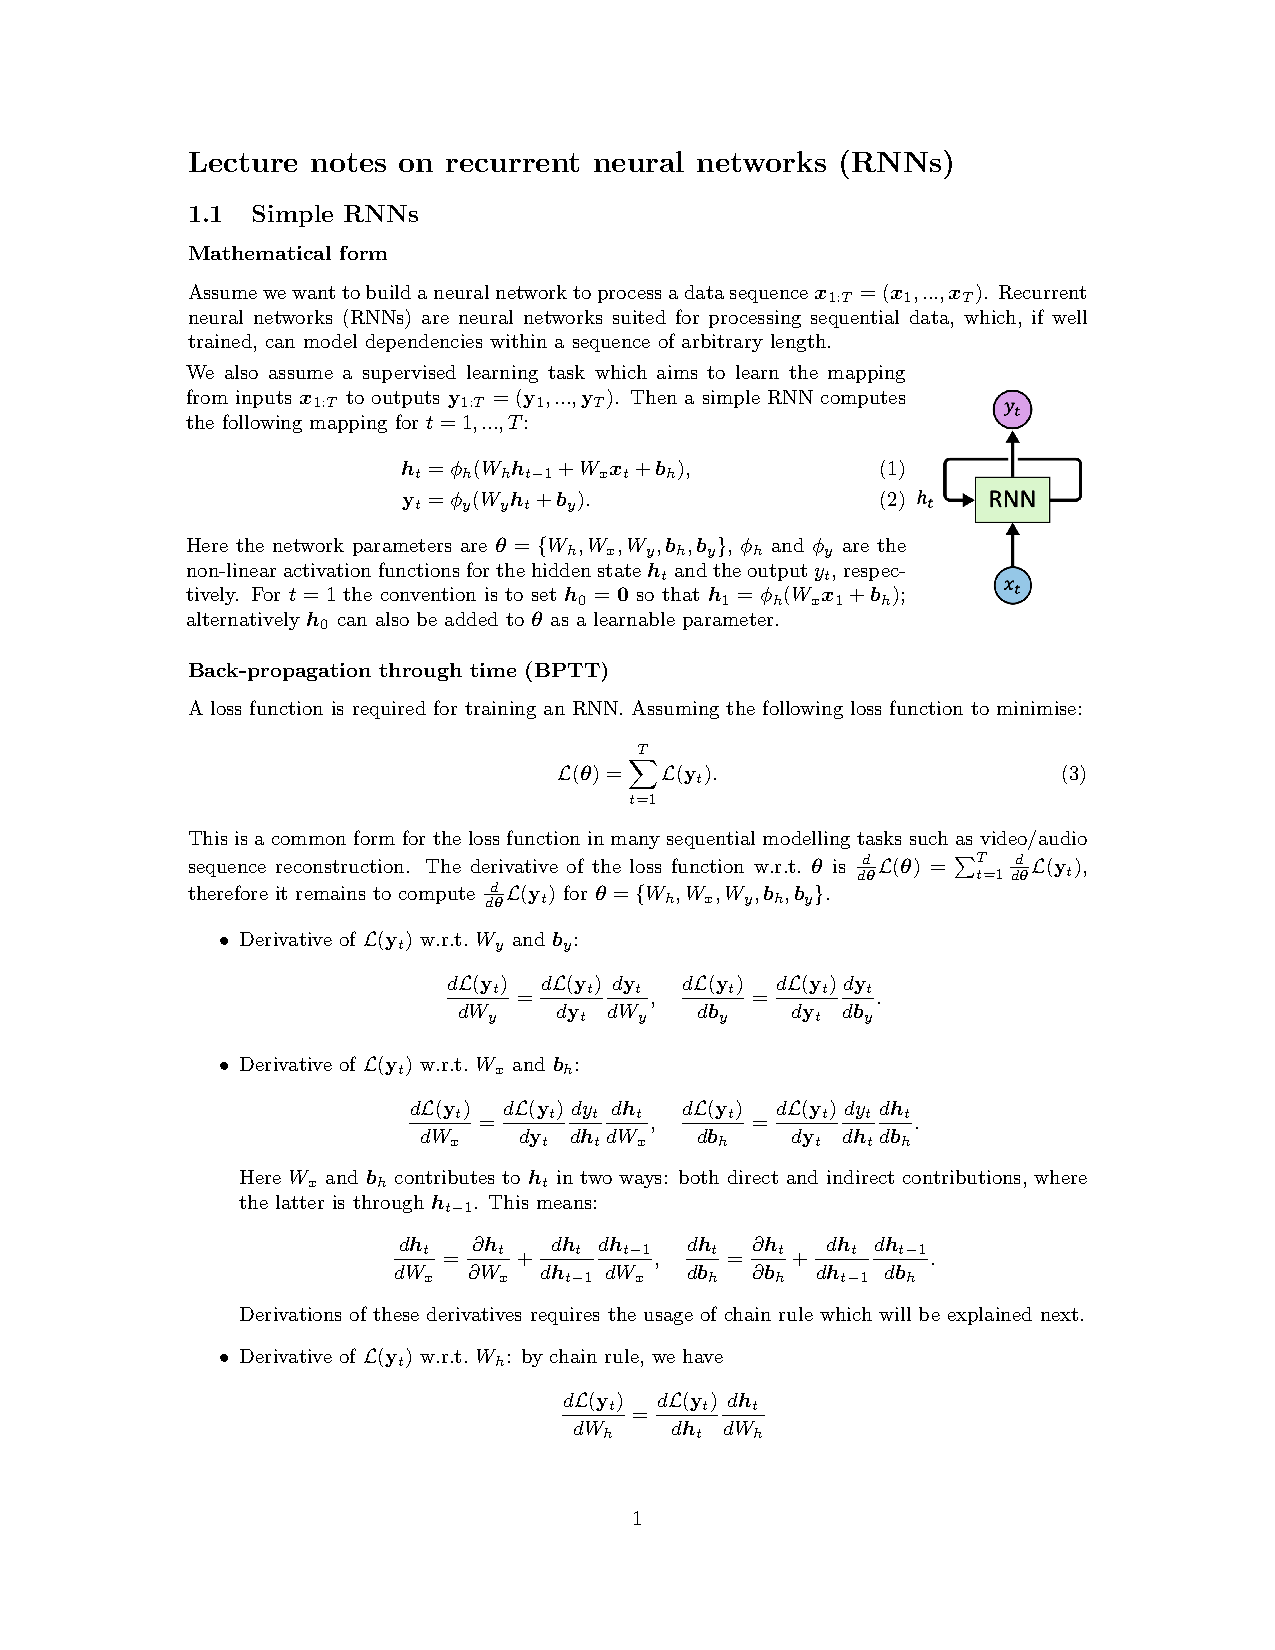
\includegraphics[page=1, trim=3cm 17cm 3cm 4.7cm, clip=true, width=.95\linewidth]{N11_RNN.pdf}}
\end{figure}

\subsection{Training RNNs}

\subsubsection{Back-propagation through time (BPTT)}

% \begin{figure}[H]
%     \centering
%     \fbox{\includegraphics[page=10, trim=1cm 2.7cm 8cm 4.5cm, clip=true, width=.95\linewidth]{L11-14_rnns.pdf}}
%     \caption*{Training the neural network}
% \end{figure}

\begin{figure}[H]
    \centering
    \fbox{\includegraphics[page=2, trim=3cm 19.5cm 3cm 2.5cm, clip=true, width=.95\linewidth]{N11_RNN.pdf}}
\end{figure}

We want to minimise the loss of $\mathcal L(\vec\theta)=L_{total}(\vec \theta)=\sum^T_{t=1}L(y_t)$ using gradient descent. This means we need to compute the gradient of the loss with respect to the parameters of the model.  

\begin{figure}[H]
    \centering
    \fbox{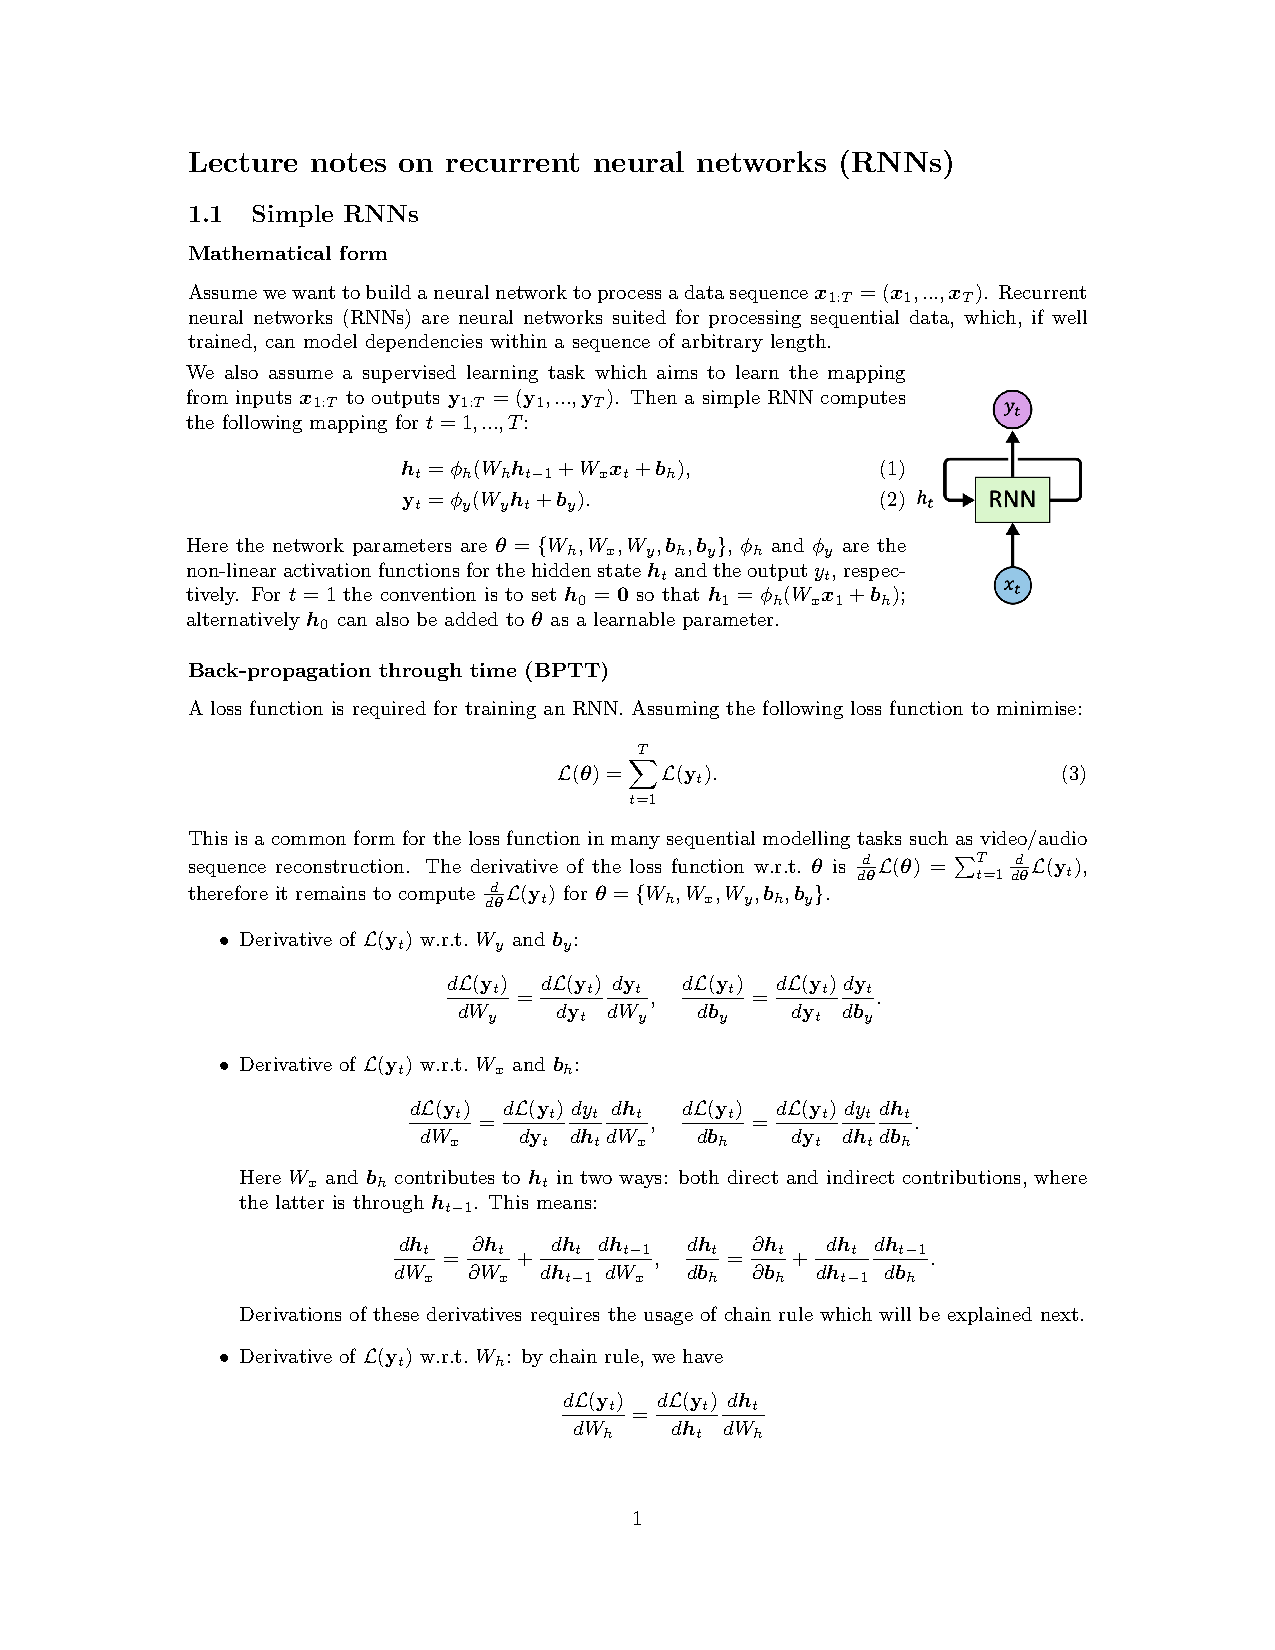
\includegraphics[page=1, trim=3cm 12.5cm 3cm 11.6cm, clip=true, width=.95\linewidth]{N11_RNN.pdf}}
\end{figure}

\begin{figure}[H]
    \centering
    \fbox{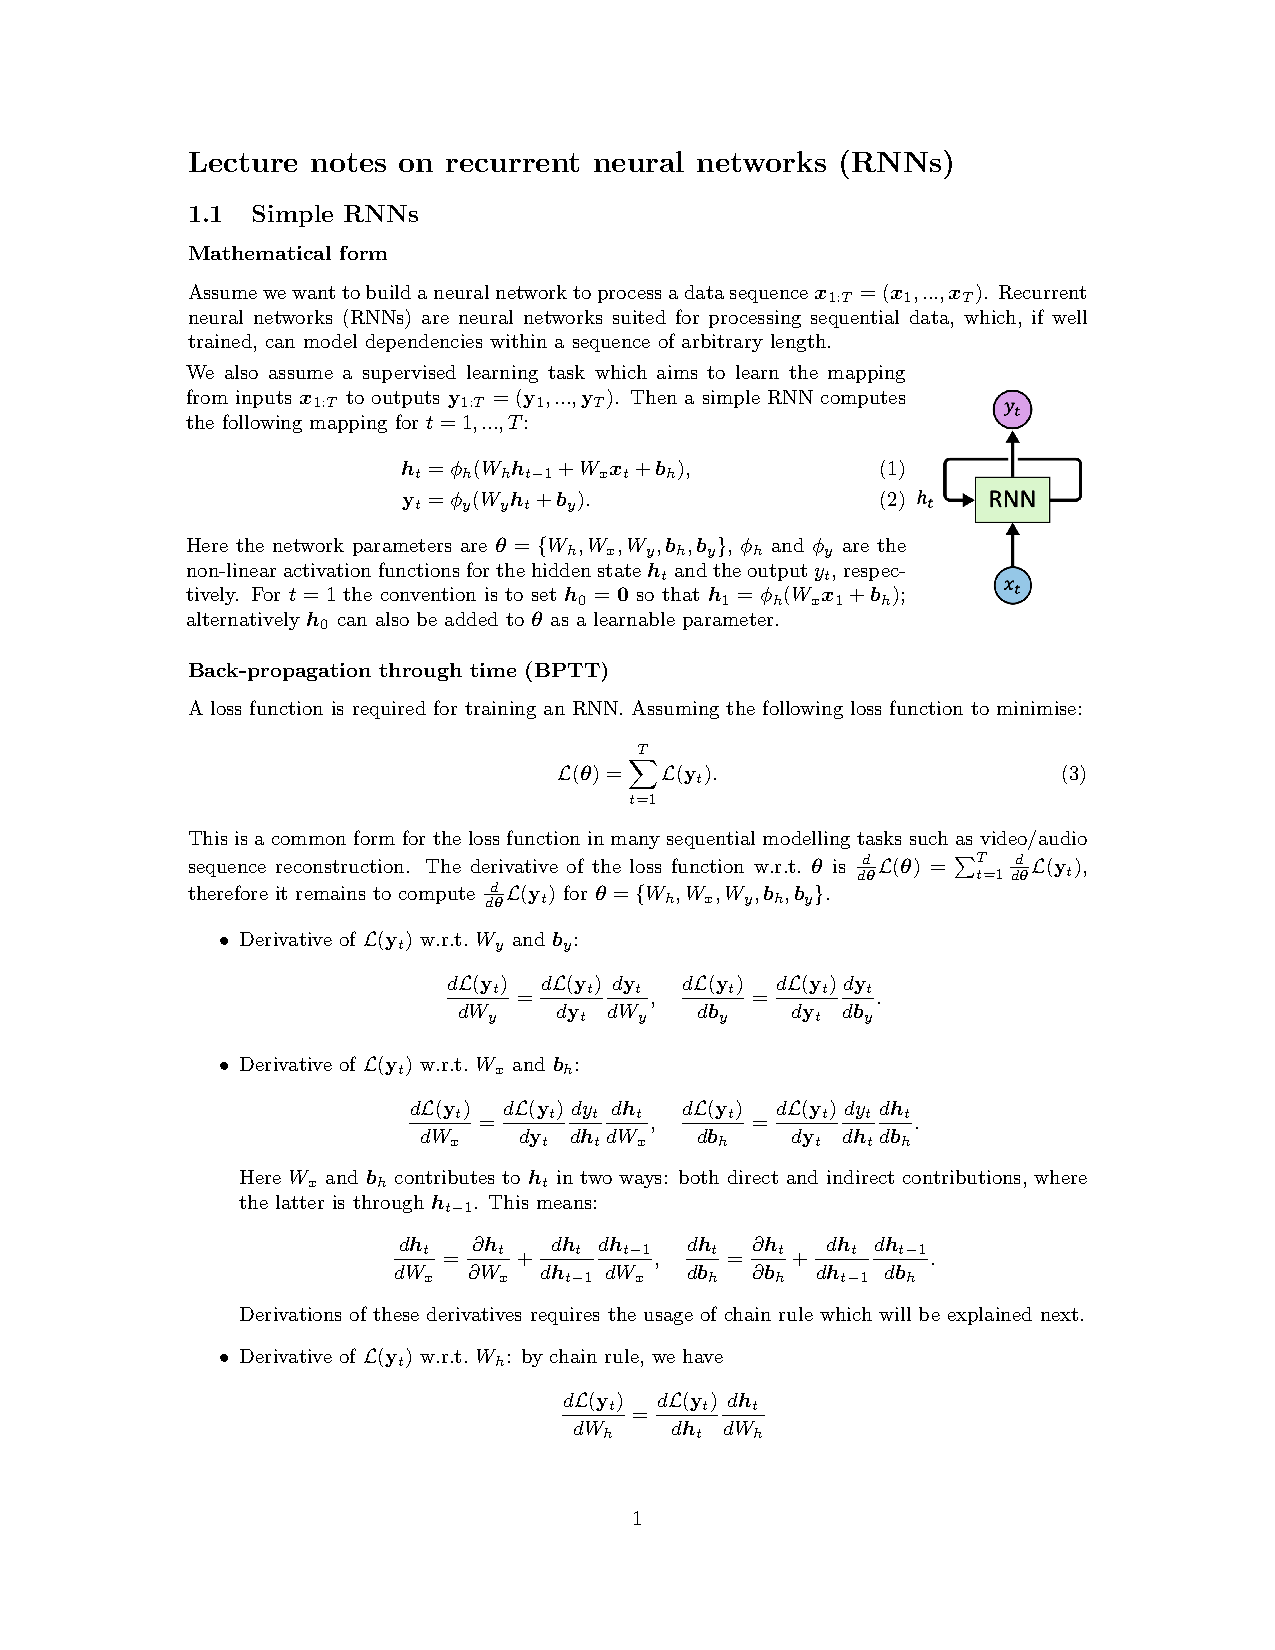
\includegraphics[page=1, trim=3cm 3.5cm 3cm 15.5cm, clip=true, width=.95\linewidth]{N11_RNN.pdf}}
\end{figure}

\begin{figure}[H]
    \centering
    \fbox{\includegraphics[page=2, trim=3cm 9cm 3cm 8.8cm, clip=true, width=.95\linewidth]{N11_RNN.pdf}}
\end{figure}

\subsubsection{Gradient vanishing/explosion issues}

Depending on the weight matrix and the activation function the product of the partial graident can vanish or explode as the number of time steps increases.

\begin{figure}[H]
    \centering
    \fbox{\includegraphics[page=2, trim=3cm 3cm 3cm 20.3cm, clip=true, width=.95\linewidth]{N11_RNN.pdf}}
    \caption*{Here, the circled dot operator is typically used to represent element-wise multiplication}
\end{figure}

\begin{figure}[H]
    \centering
    \fbox{\includegraphics[page=3, trim=3cm 15.6cm 3cm 2.5cm, clip=true, width=.95\linewidth]{N11_RNN.pdf}}
\end{figure}

Therefore, long term dependencies are getting harder to learn. With vanishing gradient, Since the gradient for $W_h$ is the sum of back-prop gradient with different window length, this gradient will be dominated especially when $t >> \tau$; the learning signal will be dominated by the short term dependencies.

\begin{figure}[H]
    \centering
    \fbox{\includegraphics[page=17, trim=3cm 3cm 4cm 11cm, clip=true, width=.95\linewidth]{L11-14_rnns.pdf}}
    % \caption*{}
\end{figure}

Tricks for how to fix the gradient vanishing or explosion issue are detailed in the Appendix~\ref{app:tricks-gradient-v/e}.

\section{Long Short-Term Memory (LSTM)}

\subsection{Forward Pass}

\begin{figure}[H]
    \centering
    \fbox{\includegraphics[page=18, trim=6cm 5.5cm 6cm 4.5cm, clip=true, width=.95\linewidth]{L11-14_rnns.pdf}}
    \caption*{Addresses the problem of gradient descent problem. They perform better at learning long-term dependencies than simple RNNs}
\end{figure}

The Long Short-term Memory was proposed with the motivation of adderssing the graident vanishing/explosion problem. It introduces memory cell states and gates to control the error flows, in detail the computation goes as follows (with $\sigma(\cdot)$ as sigmoid funciton):

\begin{figure}[H]
    \centering
    \fbox{\includegraphics[page=4, trim=3cm 19.3cm 3cm 3.3cm, clip=true, width=.95\linewidth]{N11_RNN.pdf}}
    \caption*{Here, commas (e.g.) $[h_{t-1},x_t]$ mean concatenations}
\end{figure}

\begin{figure}[H]
    \centering
    \subfigure
        [Forget gate: used to control the cell state update. It depends on the previous hidden state and current input. This is a one layer network with sigmoid activation function. Equation (7) above.]
        {
            \fbox{\includegraphics[page=19, trim=3.3cm 6.5cm 21.5cm 6.5cm, clip=true, width=.3\linewidth]{L11-14_rnns.pdf}}
    }
    \subfigure
        [The second step is to propose a cnadidate update value $\tilde{c}_t$ to the cell state. In this case an input gate is also computed to form the cell state value as well. Equations (8) and (10) above.]
        {
            \fbox{\includegraphics[page=20, trim=3.3cm 6.5cm 21.5cm 6.5cm, clip=true, width=.3\linewidth]{L11-14_rnns.pdf}}
    }
    \subfigure
        [Cell state update. $f_t$ controls the maintenance of the previous cell states. Similarly, the input gate controlls whether the candidate update will be accepted or not. Equation (11) above.]
        {
            \fbox{\includegraphics[page=21, trim=3.3cm 6.5cm 21.5cm 6.5cm, clip=true, width=.3\linewidth]{L11-14_rnns.pdf}}
    }
\end{figure}

\begin{figure}[H]
    \centering
    \subfigure
        [Finally, compute the updates for the hidden states $h_t$. Here $h_t$ is used to output a cell state $c_t$. But here, an output gate is also being used. THis means sometimes the hidden state will be 0 given the output gate values. Equations (9) and (12) above.]
        {
            \fbox{\includegraphics[page=22, trim=3.3cm 6.5cm 21.5cm 6.5cm, clip=true, width=.3\linewidth]{L11-14_rnns.pdf}}
    }
    \caption*{The Prediction of $y_t$ can proceed in a simlar way as in simple RNNS: $y_t = \Phi_y(W_yh_t + b_y)$ by transforming the hidden state $h_t$ with one neural network layer.}
\end{figure}

\subsection{Backwards Pass}

In this case, the recurrent state we care about is the cell state $c_t$. Back-prop thorugh time applies to computing the graident with respect to $W_c$ the weight matrix for computing the candidate cell state. 


\subsubsection{\color{red}{*Gradient computation}}

\begin{figure}[H]
    \centering
    \fbox{\includegraphics[page=23, trim=2.5cm 7cm 15cm 7.1cm, clip=true, width=.7\linewidth]{L11-14_rnns.pdf}}
    \caption*{``To give an idea of how this gradient is derrived, we can look at the recurrent update equation for the cell state $c_t$. Here, $c_t$ depends on $c_{t-1}$ as shown in the red box. However, there are also indirect paths via $f_t \wedge i_t \wedge c_t$ because they all depend of $h_{t-1}$ which depends on $c_{t-1}$. This gives us an idea of how to compute the total gradient.''}
\end{figure}

\begin{figure}[H]
    \centering
    \fbox{\includegraphics[page=4, trim=3cm 3cm 3cm 9.8cm, clip=true, width=.9\linewidth]{N11_RNN.pdf}}
\end{figure}

\begin{figure}[H]
    \centering
    \fbox{\includegraphics[page=5, trim=3cm 17cm 3cm 2.5cm, clip=true, width=.9\linewidth]{N11_RNN.pdf}}
\end{figure}

\subsection{How LSTMs alleviate training difficulties of RNNs}

\begin{figure}[H]
    \centering
    \fbox{\includegraphics[page=24, trim=2.4cm 1.1cm 0.5cm 4.2cm, clip=true, width=.95\linewidth]{L11-14_rnns.pdf}}
    \caption*{The usage of forget gates is useful for gradient explosion problems, becuase the network can learn a forget gate value of 0. Similarly, the product of gradients after expansion contains terms like product of $f_t$ terms times other terms. If the forget gates are open, then this term becomes the gradient of $c_{\tau+1}$ with resepect ot $h_\tau$. If $\tau$ is small and $i$ is big, then errors can also be back-propogated and doesn't vanish. This is useful for learning long-term dependencies.}
\end{figure}

\subsection{Alternatives | Gated Recurrent Unit (GRU)}

\begin{minipage}[l]{.4\linewidth}
    \begin{figure}[H]
        \centering
        \fbox{\includegraphics[page=25, trim=3cm 6.5cm 22cm 6.3cm, clip=true, width=0.95\linewidth]{L11-14_rnns.pdf}}
    \end{figure}
\end{minipage}\hfill
\begin{minipage}[r]{.55\linewidth}
    Simplified versions of the LSTM have been proposed. Compared to LSTMs, GRU only uses switching gates $z_t$ and reset gates $r_t$. you can still see that GRU still implements gating mechanisms to control the updates fo rthe recurrent states.
\end{minipage}

\begin{figure}[H]
    \centering
    \fbox{\includegraphics[page=5, trim=3cm 10.5cm 3cm 12cm, clip=true, width=.95\linewidth]{N11_RNN.pdf}}
\end{figure}

\subsubsection{LSTM vs GRU}

\begin{itemize}
    \item Other gated RNN variants exists, but LSTM and GRU are the most widely-used
    \item GRU is quicker to compute and has fewer parameters
    \item No conclusive evidence for LSTM > GRU or vice versa
    \item LSTM is a good default choice (especially if your data has particularly long dependencies, or you have lots of training data)
    \item Switch to GRU if you want more efficient compute \& less overfitting
\end{itemize}

\subsection{Stacking LSTMs}

\begin{figure}[H]
    \centering
    \fbox{\includegraphics[page=27, trim=2cm 4cm 2cm 5.3cm, clip=true, width=0.95\linewidth]{L11-14_rnns.pdf}}
\end{figure}

\subsection{Bidirectional LSTMs}

\begin{figure}[H]
    \centering
    \fbox{\includegraphics[page=28, trim=2cm 4cm 2cm 5.3cm, clip=true, width=0.95\linewidth]{L11-14_rnns.pdf}}
    \caption*{Has shown to improve performance}
\end{figure}

\section{Sequence-to-sequence models}

\begin{figure}[H]
    \centering
    \fbox{\includegraphics[page=5, trim=3cm 3cm 3cm 18.5cm, clip=true, width=.95\linewidth]{N11_RNN.pdf}}
\end{figure}

\begin{figure}[H]
    \centering
    \fbox{\includegraphics[page=6, trim=3cm 3.8cm 3cm 2.5cm, clip=true, width=.95\linewidth]{N11_RNN.pdf}}
\end{figure}

\clearpage

\appendix

\section{RNN notes}

\subsection{Tricks to fix the gradient vanishing/explosion issue}\label{app:tricks-gradient-v/e}

\begin{figure}[H]
    \centering
    \fbox{\includegraphics[page=3, trim=3cm 5.8cm 3cm 13.2cm, clip=true, width=.95\linewidth]{N11_RNN.pdf}}
\end{figure}

\subsection{Long Short-Term Memory (LSTM)}

\subsection{\color{red}{*Generative models for sequences}}

\begin{figure}[H]
    \centering
    \fbox{\includegraphics[page=7, trim=3cm 23.5cm 3cm 3.2cm, clip=true, width=.95\linewidth]{N11_RNN.pdf}}
\end{figure}

\subsubsection{Sequence VAE with global latent variables}

\begin{figure}[H]
    \centering
    \fbox{\includegraphics[page=7, trim=3cm 13.6cm 3cm 5.6cm, clip=true, width=.95\linewidth]{N11_RNN.pdf}}
\end{figure}

\subsubsection{State-space models}

\begin{figure}[H]
    \centering
    \fbox{\includegraphics[page=7, trim=3cm 3cm 3cm 15.2cm, clip=true, width=.95\linewidth]{N11_RNN.pdf}}
\end{figure}

\begin{figure}[H]
    \centering
    \fbox{\includegraphics[page=8, trim=3cm 12.5cm 3cm 2.5cm, clip=true, width=.95\linewidth]{N11_RNN.pdf}}
\end{figure}

\section{Attention Notes}

\begin{figure}[H]
    \centering
    \fbox{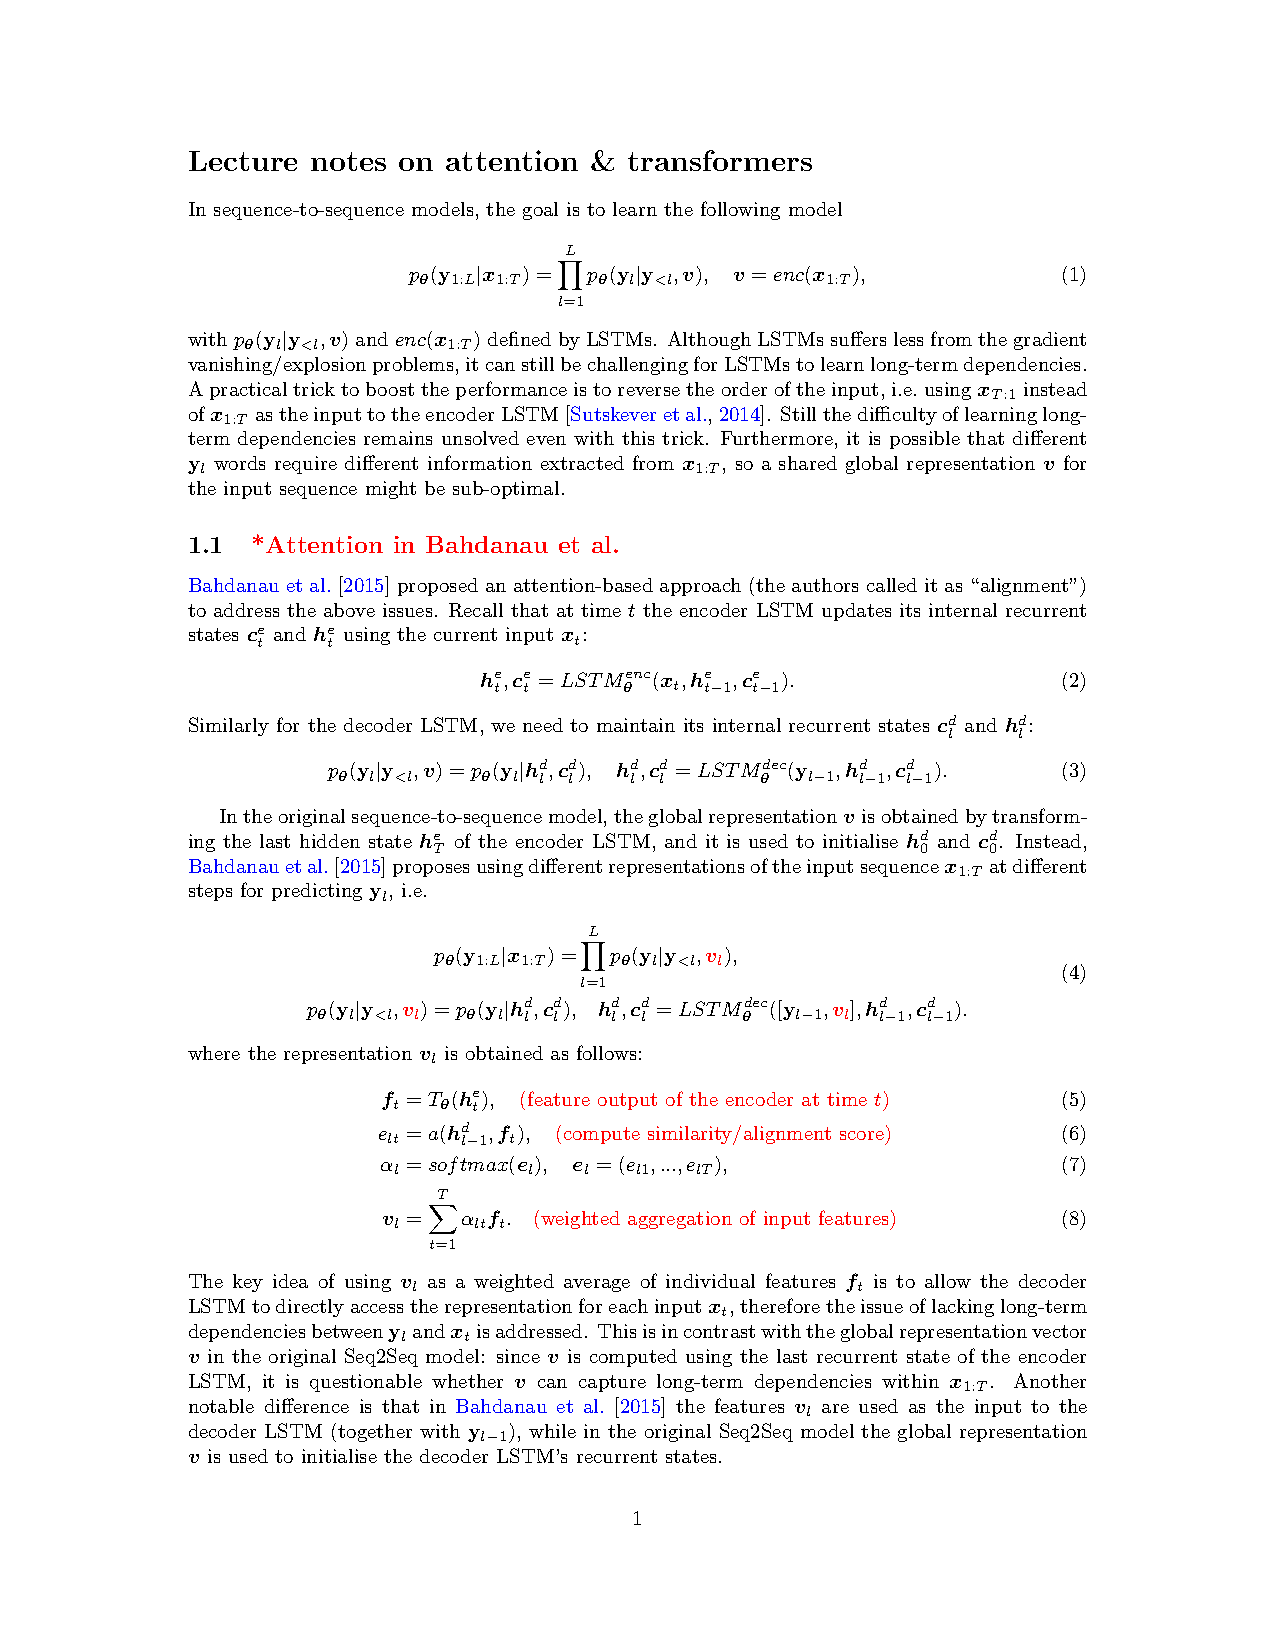
\includegraphics[page=1, trim=3cm 19.5cm 3cm 3.3cm, clip=true, width=.95\linewidth]{N13_attention.pdf}}
\end{figure}

\subsection{\color{red}{*Attention in Bahdanau et al.}}

\begin{figure}[H]
    \centering
    \fbox{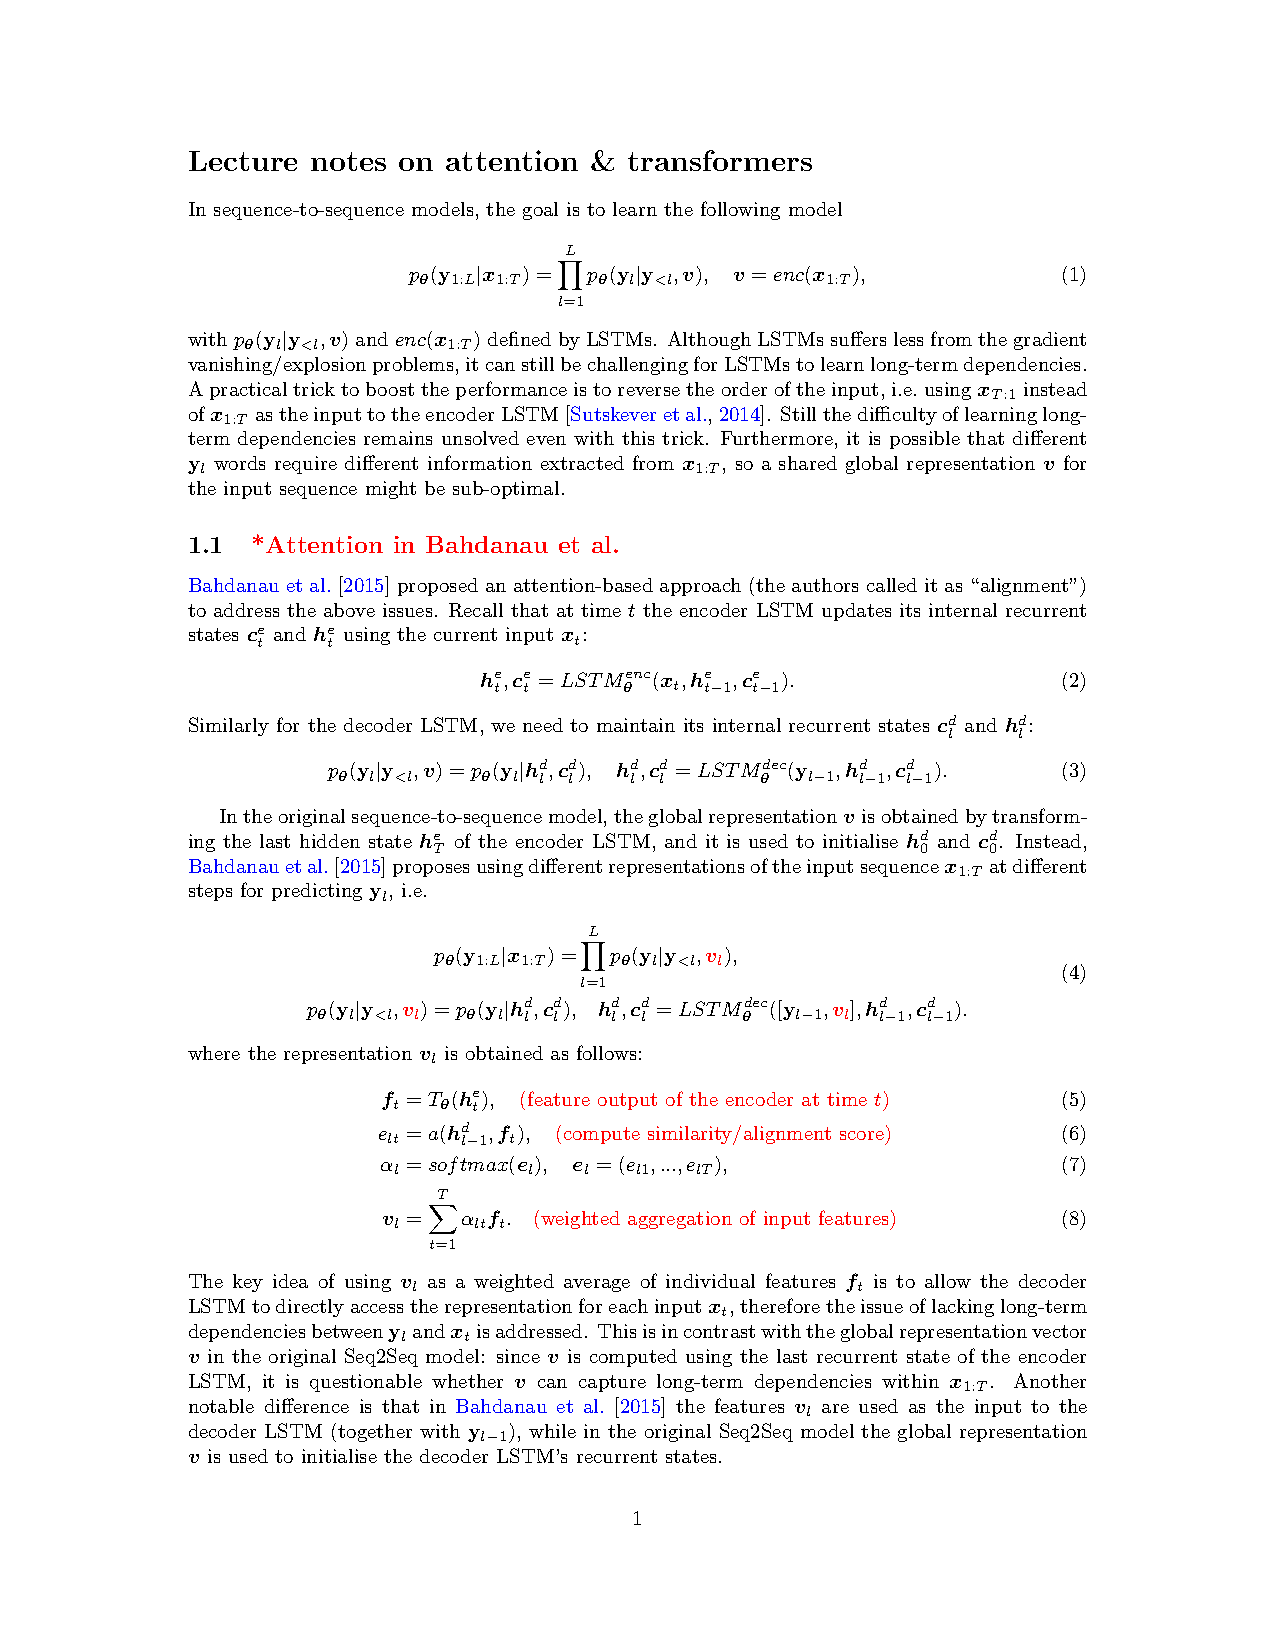
\includegraphics[page=1, trim=3cm 3cm 3cm 9.6cm, clip=true, width=.95\linewidth]{N13_attention.pdf}}
\end{figure}

\begin{figure}[H]
    \centering
    \fbox{\includegraphics[page=2, trim=3cm 23.2cm 3cm 2.5cm, clip=true, width=.95\linewidth]{N13_attention.pdf}}
\end{figure}

\subsection{Attention in transformers}

\subsubsection{Single-head attention}

\begin{figure}[H]
    \centering
    \fbox{\includegraphics[page=2, trim=3cm 5.5cm 3cm 6.5cm, clip=true, width=.95\linewidth]{N13_attention.pdf}}
\end{figure}

\subsubsection{Complexity figures}

\begin{figure}[H]
    \centering
    \fbox{\includegraphics[page=2, trim=3cm 3cm 3cm 23.5cm, clip=true, width=.95\linewidth]{N13_attention.pdf}}
\end{figure}

\begin{figure}[H]
    \centering
    \fbox{\includegraphics[page=3, trim=3cm 23.2cm 3cm 2.5cm, clip=true, width=.95\linewidth]{N13_attention.pdf}}
\end{figure}

\subsubsection{Multi-head attnetion}

\begin{figure}[H]
    \centering
    \fbox{\includegraphics[page=3, trim=3cm 10.5cm 3cm 5.8cm, clip=true, width=.95\linewidth]{N13_attention.pdf}}
\end{figure}

\subsection{Ingredients in transformers}

\begin{figure}[H]
    \centering
    \fbox{\includegraphics[page=3, trim=3cm 8.5cm 3cm 18.5cm, clip=true, width=.95\linewidth]{N13_attention.pdf}}
\end{figure}

\subsubsection{Position encoding}

\begin{figure}[H]
    \centering
    \fbox{\includegraphics[page=3, trim=3cm 3cm 3cm 20.5cm, clip=true, width=.95\linewidth]{N13_attention.pdf}}
\end{figure}

\begin{figure}[H]
    \centering
    \fbox{\includegraphics[page=4, trim=3cm 5.7cm 3cm 2.5cm, clip=true, width=.95\linewidth]{N13_attention.pdf}}
\end{figure}

\subsubsection{Layer normalization}

\begin{figure}[H]
    \centering
    \fbox{\includegraphics[page=4, trim=3cm 3.3cm 3cm 23.2cm, clip=true, width=.95\linewidth]{N13_attention.pdf}}
\end{figure}

\begin{figure}[H]
    \centering
    \fbox{\includegraphics[page=5, trim=3cm 22cm 3cm 2.5cm, clip=true, width=.95\linewidth]{N13_attention.pdf}}
\end{figure}

\subsubsection{Point-wise feed-forward network}

\begin{figure}[H]
    \centering
    \fbox{\includegraphics[page=5, trim=3cm 19cm 3cm 6.8cm, clip=true, width=.95\linewidth]{N13_attention.pdf}}
\end{figure}


% \printbibliography
% \addcontentsline{toc}{section}{Bibliography}

\end{document}